\chapter{Requirement specification}
\textit{The requirement specification is focused around the CDU and the sensor node. It describes the functionality requirements along with other general requirements.}
\section{General description}
Below on figure \ref{fig:project_system} the system is shown. The focus of the requirement specification will be upon the elements shown in this figure.
\begin{figure}[H]
	\centering
	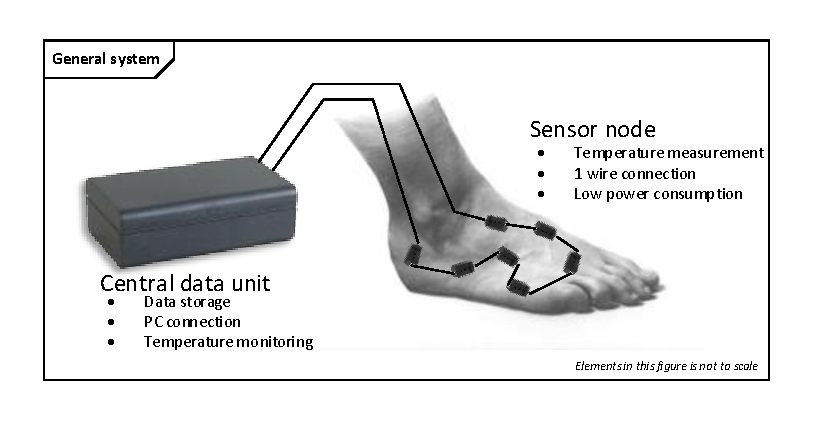
\includegraphics[width=.9\textwidth]{billeder/7requirementspec/GeneralSystem}
	\caption{Project system}
	\label{fig:project_system}
\end{figure}
The system will be mounted on and around the foot of a person who is likely to develop charcot foot. 
\section{Functionality requirements}
The sensor system has two main functionalities:
\begin{enumerate}
	\item Set system to normal operation
	\item Extract data from CDU
\end{enumerate}
These use cases handles the expected normal functionality as seen from the end user. The users/actors of the system can be found in table \ref{tab:actors}.
\begin{table}[H]
	\centering
	\begin{tabular}{|l|l|p{9.5cm}|}
	\hline
	Actor name & Type & Description \\ \hline
	Patient & Primary & The patient set the system to run and initiates data extraction from the CDU. \\ \hline
	Computer & Secondary  & The computer can extract data from the Central data unit. It is not intended as a control unit but mostly just for demonstration and debug purposes.\\ \hline
	\end{tabular}
	\caption{Actors of the system}
	\label{tab:actors}
\end{table}
The use case set system to normal operation has the responsibility to power on the system and set it to normal operation mode. It is initiated by the patient actor.\\
The use case extract data from CDU has the responsibility to move the stored data from the CDU to a piece of computer software. It is initiated by the patient actor and has a computer as the secondary actor. 
\begin{figure}[H]
	\centering
	\includegraphics[width=.7\textwidth]{billeder/7requirementspec/usecase_vector}
	\caption{Use case diagram}
\end{figure}
For the full use cases see the requirement specification document.
\section{General requirements}
\textit{This section seeks to explain the most important general requirements of the system}.
\subsection{Functionality requirements}
\begin{table}[H]
\begin{tabular}{p{8cm} p{2cm}}
$\bullet$ Cycle: & 1 min\\
\end{tabular}
\end{table}
A cycle must include collecting data from every sensor connected to the bus. This can also be understood as the CDU must collect the overall temperature or other data every minute.\\
The data must be saved to memory which leads to the following requirement:
\begin{table}[H]
\begin{tabular}{p{8cm} p{5cm}}
$\bullet$ Memory: & 24 hours of data collection ($\sim$152kB) 256kB suggested.\\
$\bullet$ Real time clock: & Yes\\
$\bullet$ Save entries must contain: &Sensor identifier. \\
~ 									&Temperature. \\
~									&Timestamp. \\
~									&Type. \\
~									&Erros. \\
\end{tabular}
\end{table}
A real time clock must be used in order to acquire the timestamp needed in the save entries. The type of the sensor is hard coded into the device.
\subsection{Power consumption}
In order to comply with the original idea of the system, a demand for low power consumption has made. The power consumption requirements are based on rough estimates made by the group. The power consumption requirements are as follows:
\begin{table}[H]
	\begin{tabular}{p{8cm} p{2cm}}
	$\bullet$ CDU Power consumption: & <0.5W\\
	$\bullet$ Sensor node Power consumption: & <0.05W\\
	\end{tabular}
\end{table}
The CDU power consumption requirement is excluding the sensor node power consumption.
\subsection{Interface requirements}
In the central data unit requirements part of the general requirement section in the requirement specification document it is stated that the external interfaces must be:
\begin{table}[H]
	\begin{tabular}{p{8cm} p{2cm}}
	$\bullet$ Custom power line communication bus: & Yes\\
	$\bullet$ CDU to computer interface: & Yes\\
	\end{tabular}
\end{table}
The sensor nodes require the Custom power line communication bus as an external interface as well. These non-constricting requirements make room for a lot of different design opportunities.
%\subsection{Other requirements}
%A BOM (Build of Materials) price have been specified in the requirements. The original project formulation specifies a need for minimising the production cost. The price is rather high as it serves as food for thought. The production price still has unknown elements like assembly cost which is why a materials price have been specified.